\documentclass[8pt, xcolor={svgnames}, hyperref={linkcolor=black}]{beamer}
\usetheme[progressbar=frametitle]{metropolis}
\setbeamerfont{footnote}{size=\tiny}
\usepackage{appendixnumberbeamer}
\usepackage{url}
\usepackage{amsfonts} 
\usepackage{amssymb}
\usepackage[english]{babel}
\usepackage{fontawesome}
\usepackage{multicol}
\usepackage{bm}
\usepackage{braket}
\usepackage{algorithm}
\usepackage{algpseudocode}
\usepackage{enumitem}

\usepackage[]{pseudo}

\usepackage{tikz}
\usetikzlibrary{positioning,arrows,calc,math,angles,quotes}

\usetikzlibrary{arrows,automata}
\usetikzlibrary{positioning}
\usetikzlibrary{arrows.meta,
                bending,
                intersections,
                quotes,
                shapes.geometric}

\tikzset{
    state/.style={
           rectangle,
           rounded corners,
           draw=black, very thick,
           minimum height=1em,
           inner sep=2pt,
           text centered,
           },
}

\definecolor{cadmiumgreen}{rgb}{0.0, 0.42, 0.24}
\definecolor{amethyst}{rgb}{0.6, 0.4, 0.8}

\usepackage[most]{tcolorbox}
\usepackage{xcolor}


\title{Full-Stack Quantum Machine Learning}
\date{28 September 2023}
\author{Matteo Robbiati}
\titlegraphic{
   \begin{tikzpicture}[overlay, remember picture]
   \node[at=(current page.south east), anchor=south east] {%
      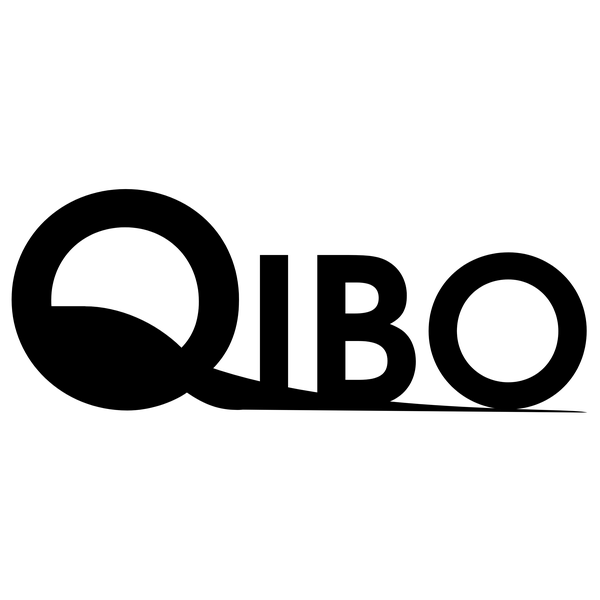
\includegraphics[width=.18\textwidth]{figures/qibo.png} 
      
\includegraphics[width=.18\textwidth]{figures/unimi.png} 
      
\includegraphics[width=.18\textwidth]{figures/cern.png}  
      
\includegraphics[width=.18\textwidth]{figures/qti.png}  
   };
   \end{tikzpicture}
}

\begin{document}

\begin{frame}
\maketitle
\end{frame}

\section{Introduction to concepts}

\begin{frame}{Machine Learning}

Machine Learning helps in solving statistical problems, such as data generation, 
classification, regression, forecasting, etc.
\pause

\begin{itemize}
\item[\faCrosshairs] we aim to know some hidden law between two variables: $\bm{y}=f(\bm{x})$;
\pause
\item[\faBarChart] we define a parameteric model with returns $\bm{y}_{\rm est}=f_{\rm est}(\bm{x}; \bm{\theta})$;
\pause
\item[\faBinoculars] we define an optimizer, which task is to compute 
   $\text{argmin}_{\bm{\theta}}\bigl[J(\bm{y}_{\rm meas}, \bm{y}_{\rm est})\bigr]$.
\end{itemize}
\pause
\begin{figure}  
    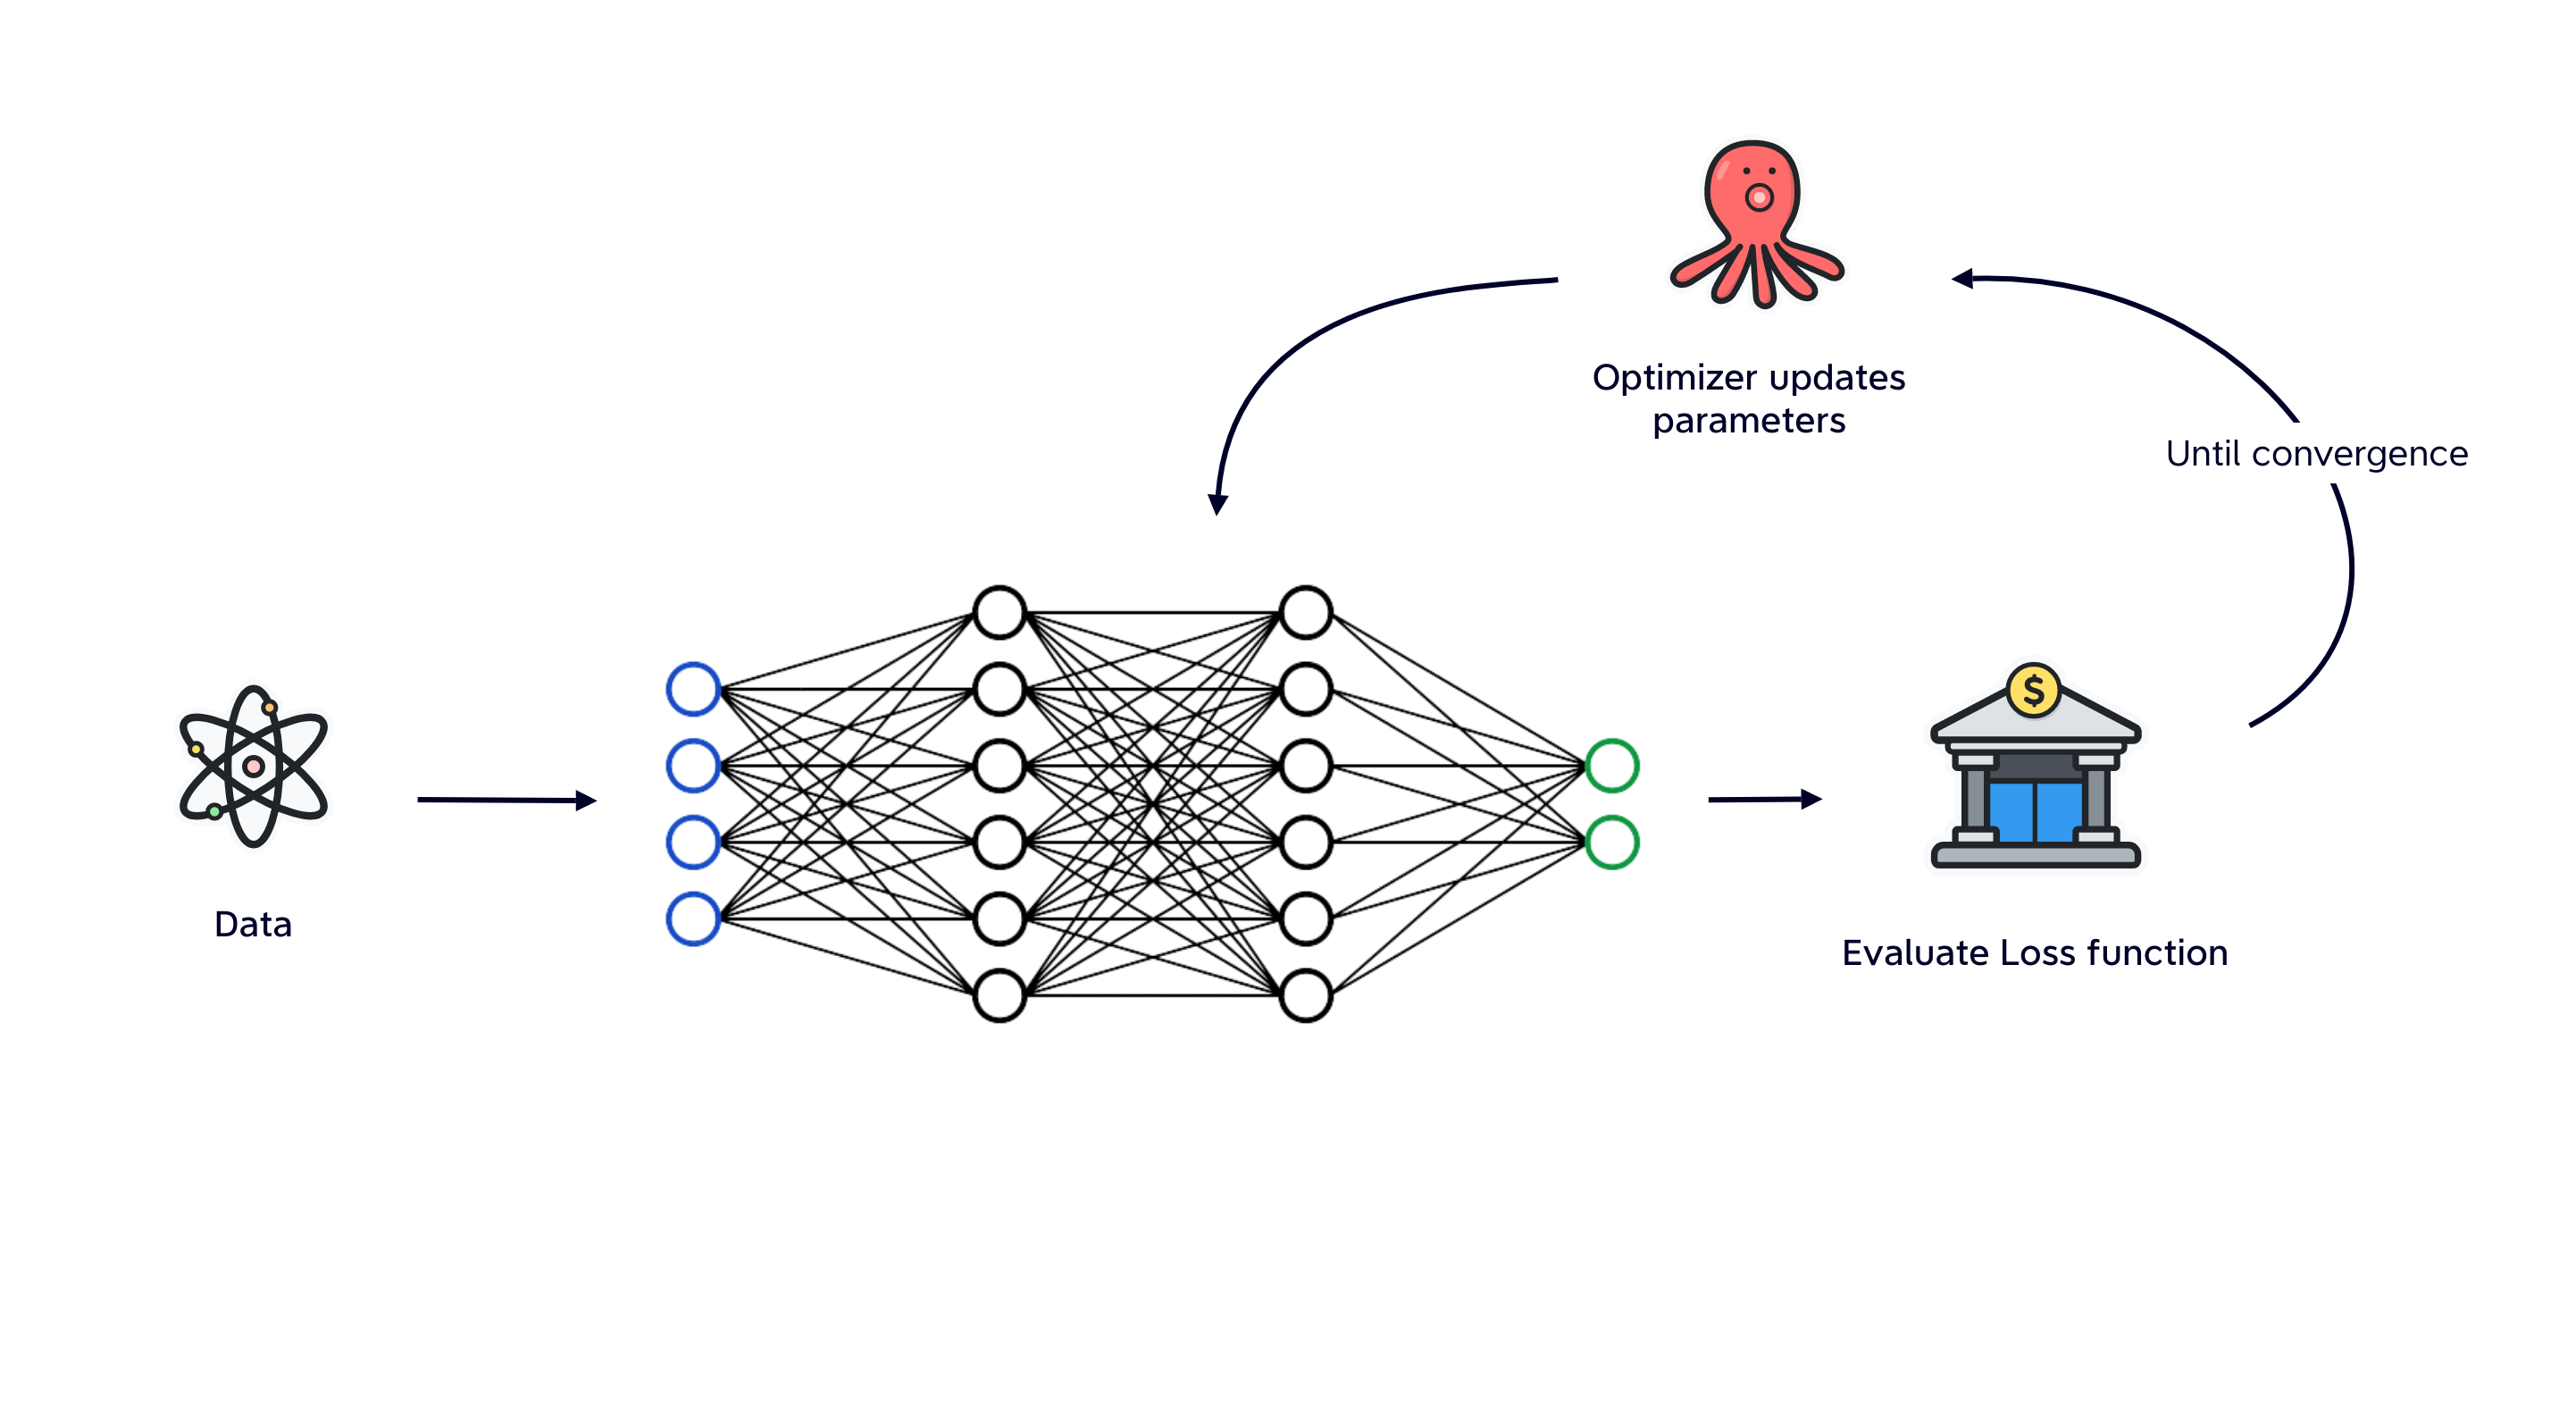
\includegraphics[width=1\textwidth]{figures/ml_scheme.png}
\end{figure}
\end{frame}

\begin{frame}{Parametric Quantum Circuits}
\pause
  \begin{itemize}
  \item<2,3,4>[\faMagic] Classical bits are replaced by \textbf{qubits}: 
  $\ket{q}=\alpha_0 \ket{0} + \alpha_1 \ket{1}$;  
  \item<3,4>[\faCog] we modify the qubits state by applying unitaries, which we call \textbf{gates}.\\
  Rotational gates $R_j(\theta)=e^{-i\theta\hat{\sigma}_j}$ are used to build
  parametric circuits $\mathcal{C}(\bm{\theta})$;
  \item<4>[\faEye] information is accessed calculating expected values $\text{E}[\hat{O}\,]$
  of target observables $\hat{O}$ on the state obtained executing $\mathcal{C}$.
  \end{itemize}
    \begin{figure}
       \includegraphics<2>[width=0.8\textwidth]{figures/vqc_1.png}
       \includegraphics<3>[width=0.8\textwidth]{figures/vqc_2.png}
       \includegraphics<4>[width=0.8\textwidth]{figures/vqc.png}   
    \end{figure}
\end{frame}

\section{Quantum Machine Learning}

% SLIDE 1 QML
\begin{frame}{Quantum Machine Learning - doing ML using QC}

\vspace{1.05cm}

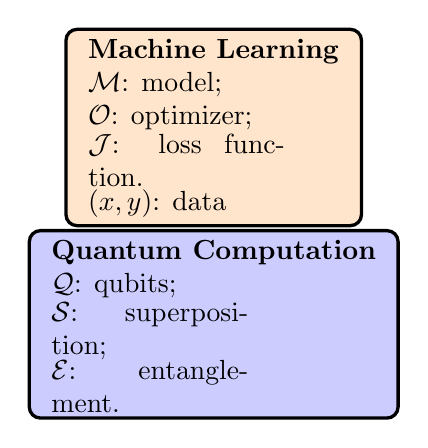
\begin{tikzpicture}[->,>=stealth']

 \node[state, fill=orange!20] (ML) 
 {\begin{tabular}{l}
 \textbf{Machine Learning}\\ 
 \parbox{2.5cm}{$\mathcal{M}$: model;}\\
 \parbox{2.5cm}{$\mathcal{O}$: optimizer;}\\
 \parbox{2.5cm}{$\mathcal{J}$: loss function.}\\
 \parbox{2.5cm}{$(x, y)$: data}
  \end{tabular}
  };
  
  \node[state,
  below of = ML,
  yshift=-1.5cm, fill=blue!20] (QC) 
 {\begin{tabular}{l}
 \textbf{Quantum Computation}\\ 
 \parbox{2.5cm}{$\mathcal{Q}$: qubits;} \\
 \parbox{2.5cm}{$\mathcal{S}$: superposition;}\\
 \parbox{2.5cm}{$\mathcal{E}$: entanglement.}
  \end{tabular}
  };
  
\end{tikzpicture}
\end{frame}


% SLIDE 2 QML
\begin{frame}{Quantum Machine Learning - operating on qubits}

\vspace{1.77cm}

\begin{tikzpicture}[->,>=stealth']

 \node[state, fill=orange!20] (ML) 
 {\begin{tabular}{l}
 \textbf{Machine Learning}\\ 
 \parbox{2.5cm}{$\mathcal{M}$: model;}\\
 \parbox{2.5cm}{$\mathcal{O}$: optimizer;}\\
 \parbox{2.5cm}{$\mathcal{J}$: loss function.}\\
 \parbox{2.5cm}{$(x, y)$: data}
  \end{tabular}
  };
  
  \node[state,
  below of = ML,
  yshift=-1.5cm, fill=blue!20] (QC) 
 {\begin{tabular}{l}
 \textbf{Quantum Computation}\\ 
 \parbox{2.5cm}{$\mathcal{Q}$: qubits;} \\
 \parbox{2.5cm}{$\mathcal{S}$: superposition;}\\
 \parbox{2.5cm}{$\mathcal{E}$: entanglement.}
  \end{tabular}
  };
  
 \node[state,
    right of=QC,
    yshift=-0.5cm,
    anchor=center,
    node distance=4.5cm, 	
    text width=3.5cm, fill=blue!20] (VQC) 
 {%
 \begin{tabular}{l}
  \textbf{Circuit execution} \\
  \parbox{4.5cm}{
  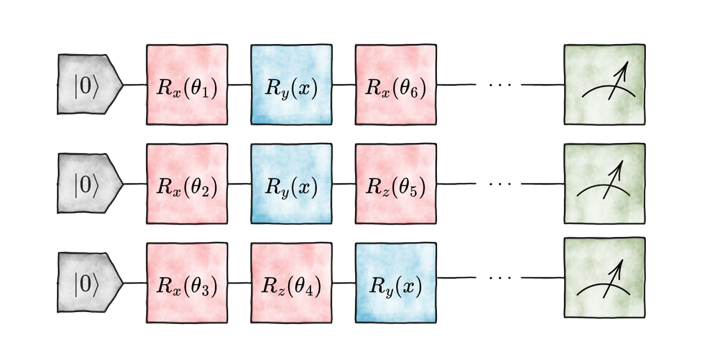
\includegraphics[width=0.9\textwidth]{figures/vqc.png}
  }
 \end{tabular}
 };
 
  \draw[line width=0.3mm] (1, -2.5)  to[out=0, in=200] (3, -3.2);
\end{tikzpicture}

\end{frame}

% SLIDE 3 QML
\begin{frame}{Quantum Machine Learning - natural randomness}

\vspace{1.77cm}

\begin{tikzpicture}[->,>=stealth']

 \node[state, fill=orange!20] (ML) 
 {\begin{tabular}{l}
 \textbf{Machine Learning}\\ 
 \parbox{2.5cm}{$\mathcal{M}$: model;}\\
 \parbox{2.5cm}{$\mathcal{O}$: optimizer;}\\
 \parbox{2.5cm}{$\mathcal{J}$: loss function.}\\
 \parbox{2.5cm}{$(x, y)$: data}
  \end{tabular}
  };
  
  \node[state,
  below of = ML,
  yshift=-1.5cm, fill=blue!20] (QC) 
 {\begin{tabular}{l}
 \textbf{Quantum Computation}\\ 
 \parbox{2.5cm}{$\mathcal{Q}$: qubits;} \\
 \parbox{2.5cm}{$\mathcal{S}$: superposition;}\\
 \parbox{2.5cm}{$\mathcal{E}$: entanglement.}
  \end{tabular}
  };
  
 \node[state,
    right of=QC,
    yshift=-0.5cm,
    anchor=center,
    node distance=4.5cm, 	
    text width=3.5cm, fill=blue!20] (VQC) 
 {%
 \begin{tabular}{l}
  \textbf{Circuit execution} \\
  \parbox{4.5cm}{
  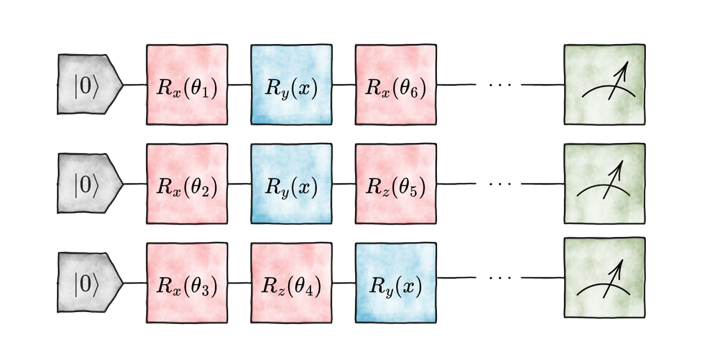
\includegraphics[width=0.9\textwidth]{figures/vqc.png}
  }
 \end{tabular}
 };
 
\node[state,
  right of = VQC,
  node distance = 3cm,
  yshift=2cm, 
  fill=blue!20] (NSHOT) 
 {\begin{tabular}{l}
 \textbf{Expected values}\\ 
 $y_{est} \equiv \braket{q_f|\hat{O}|q_f}$
  \end{tabular}
  };
 
\draw[line width=0.3mm] (1, -2.5)  to[out=0, in=200] (3, -3.2);
\draw[line width=0.3mm] (6, -2.8)  to[out=0, in=250] (7, -1.6);
\end{tikzpicture}

\end{frame}


% SLIDE 4 QML
\begin{frame}{Quantum Machine Learning - encoding the problem}

\vspace{0.56cm}
\begin{tikzpicture}[->,>=stealth']

 \node[state, fill=orange!20] (ML) 
 {\begin{tabular}{l}
 \textbf{Machine Learning}\\ 
 \parbox{2.5cm}{$\mathcal{M}$: model;}\\
 \parbox{2.5cm}{$\mathcal{O}$: optimizer;}\\
 \parbox{2.5cm}{$\mathcal{J}$: loss function.}\\
 \parbox{2.5cm}{$(x, y)$: data}
  \end{tabular}
  };
  
  \node[state,
  below of = ML,
  yshift=-1.5cm, fill=blue!20] (QC) 
 {\begin{tabular}{l}
 \textbf{Quantum Computation}\\ 
 \parbox{2.5cm}{$\mathcal{Q}$: qubits;} \\
 \parbox{2.5cm}{$\mathcal{S}$: superposition;}\\
 \parbox{2.5cm}{$\mathcal{E}$: entanglement.}
  \end{tabular}
  };
  
 
 \node[state,
    right of=QC,
    yshift=-0.5cm,
    anchor=center,
    node distance=4.5cm, 	
    text width=3.5cm, fill=blue!20] (VQC) 
 {%
 \begin{tabular}{l}
  \textbf{Circuit execution} \\
  \parbox{4.5cm}{
  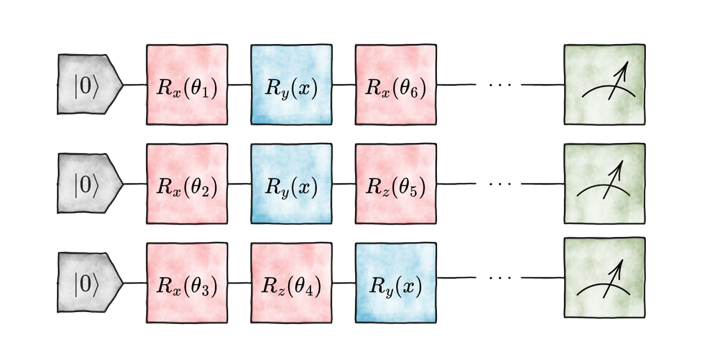
\includegraphics[width=0.9\textwidth]{figures/vqc.png}
  }
 \end{tabular}
 };
 
\node[state,
  right of = VQC,
  node distance = 3cm,
  yshift=2cm, 
  fill=blue!20] (NSHOT) 
 {\begin{tabular}{l}
 \textbf{Expected values}\\ 
 $y_{est} \equiv \braket{q_f|\hat{O}|q_f}$
  \end{tabular}
  };

  
 \draw[line width=0.3mm, red, opacity = 0.7] (0.5, 0.4)  to[out=0, in=230] (3, -3.3);
 \draw[line width=0.3mm, orange, opacity = 0.7] (-1.2, -1.25)  to[out=260, in=300] (4.4, -4.1);
 \draw[line width=0.3mm, cadmiumgreen, opacity = 0.7] (-0.4, -1.2)  to[out=330, in=80] (7.8, -0.4);
  
 
 \draw[red, line width=0.4mm, opacity = 0.9] (-1.1, 0.4) circle (0.4 cm);
 \draw[cadmiumgreen, line width=0.4mm, opacity = 0.9] (-0.65,-0.8) circle (0.3 cm);
 \draw[cadmiumgreen, line width=0.4mm, opacity = 0.9] (7.2,-1.4) rectangle (8.6, -0.95);
 \draw[orange, line width=0.4mm, opacity = 0.6] (-1.15,-0.8) circle (0.3 cm);
 \draw[red, line width=0.4mm, opacity = 0.6] (3.1,-4) rectangle (6,-2.4);
 \draw[orange, line width=0.4mm, opacity = 0.9] (3.5,-3.9) rectangle (5.2,-2.5);


\end{tikzpicture}
\end{frame}


% SLIDE 5 QML
\begin{frame}{Quantum Machine Learning!}

\vspace{0.42cm}
\begin{tikzpicture}[->,>=stealth']


 \node[state, fill=orange!20] (ML) 
 {\begin{tabular}{l}
 \textbf{Machine Learning}\\ 
 \parbox{2.5cm}{$\mathcal{M}$: model;}\\
 \parbox{2.5cm}{$\mathcal{O}$: optimizer;}\\
 \parbox{2.5cm}{$\mathcal{J}$: loss function.}\\
 \parbox{2.5cm}{$(x, y)$: data}
  \end{tabular}
  };
  
  \node[state,
  below of = ML,
  yshift=-1.5cm, fill=blue!20] (QC) 
 {\begin{tabular}{l}
 \textbf{Quantum Computation}\\ 
 \parbox{2.5cm}{$\mathcal{Q}$: qubits;} \\
 \parbox{2.5cm}{$\mathcal{S}$: superposition;}\\
 \parbox{2.5cm}{$\mathcal{E}$: entanglement.}
  \end{tabular}
  };
  

 \node[state,   
  text width=3cm, 
  yshift=1.5cm, 
  right of=ML, 	
  node distance=4cm, 
  anchor=center, fill=green!20] (OPT) 
 {%
 \begin{tabular}{l} 	% content
  \textbf{Optimizer $\mathcal{O}$}\\
  Hybrid-strategy
 \end{tabular}
 };
 
 \node[state,
    right of=QC,
    yshift=-0.5cm,
    anchor=center,
    node distance=4.5cm, 	
    text width=3.5cm, fill=blue!20] (VQC) 
 {%
 \begin{tabular}{l}
  \textbf{Circuit execution} \\
  \parbox{4.5cm}{
  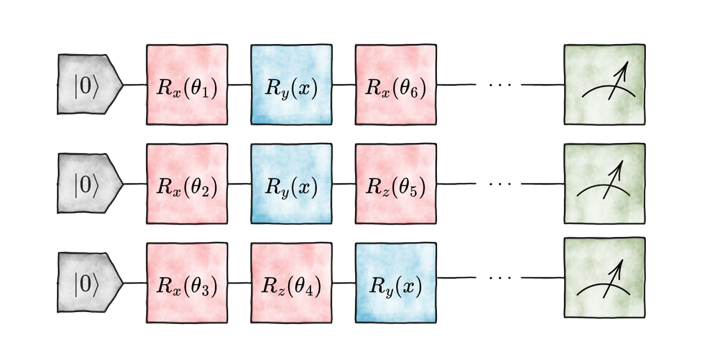
\includegraphics[width=0.9\textwidth]{figures/vqc.png}
  }
 \end{tabular}
 };
 
\node[state,
  right of = VQC,
  node distance = 3cm,
  yshift=2cm, 
  fill=blue!20] (NSHOT) 
 {\begin{tabular}{l}
 \textbf{Expected values}\\ 
 $y_{est} \equiv \braket{q_f|\hat{O}|q_f}$
  \end{tabular}
  };
  
  \node[state,
  above of = NSHOT,
  node distance = 1.5cm,
  yshift=0cm, fill=green!20] (J) 
 {\begin{tabular}{l}
 \textbf{loss function $\mathcal{J}$}\\ 
 $\mathcal{J}(y_{meas}, y_{est})$
  \end{tabular}
  };
  

 \draw[line width=0.3mm] (6.5, -3)  to[out=0, in=270] (7.5, -1.6);
 \draw[line width=0.3mm] (6, -1.1)  to[out=180, in=200] (6.1, 0.2);
 \draw[line width=0.3mm] (7.5, 1.1)  to[out=90, in=0] (5.7, 1.5);
 \draw[line width=0.6mm, opacity=0.8] (2, 1.6)  to[out=180, in=270] (-0.2, 2.9);
 
 \draw[line width=0.3mm, orange, opacity = 0.0] (-1.2, -1.25)  to[out=260, in=300] (4.4, -3.5);

\end{tikzpicture}
\end{frame}

\begin{frame}{From ML to QML}
\begin{figure}  
   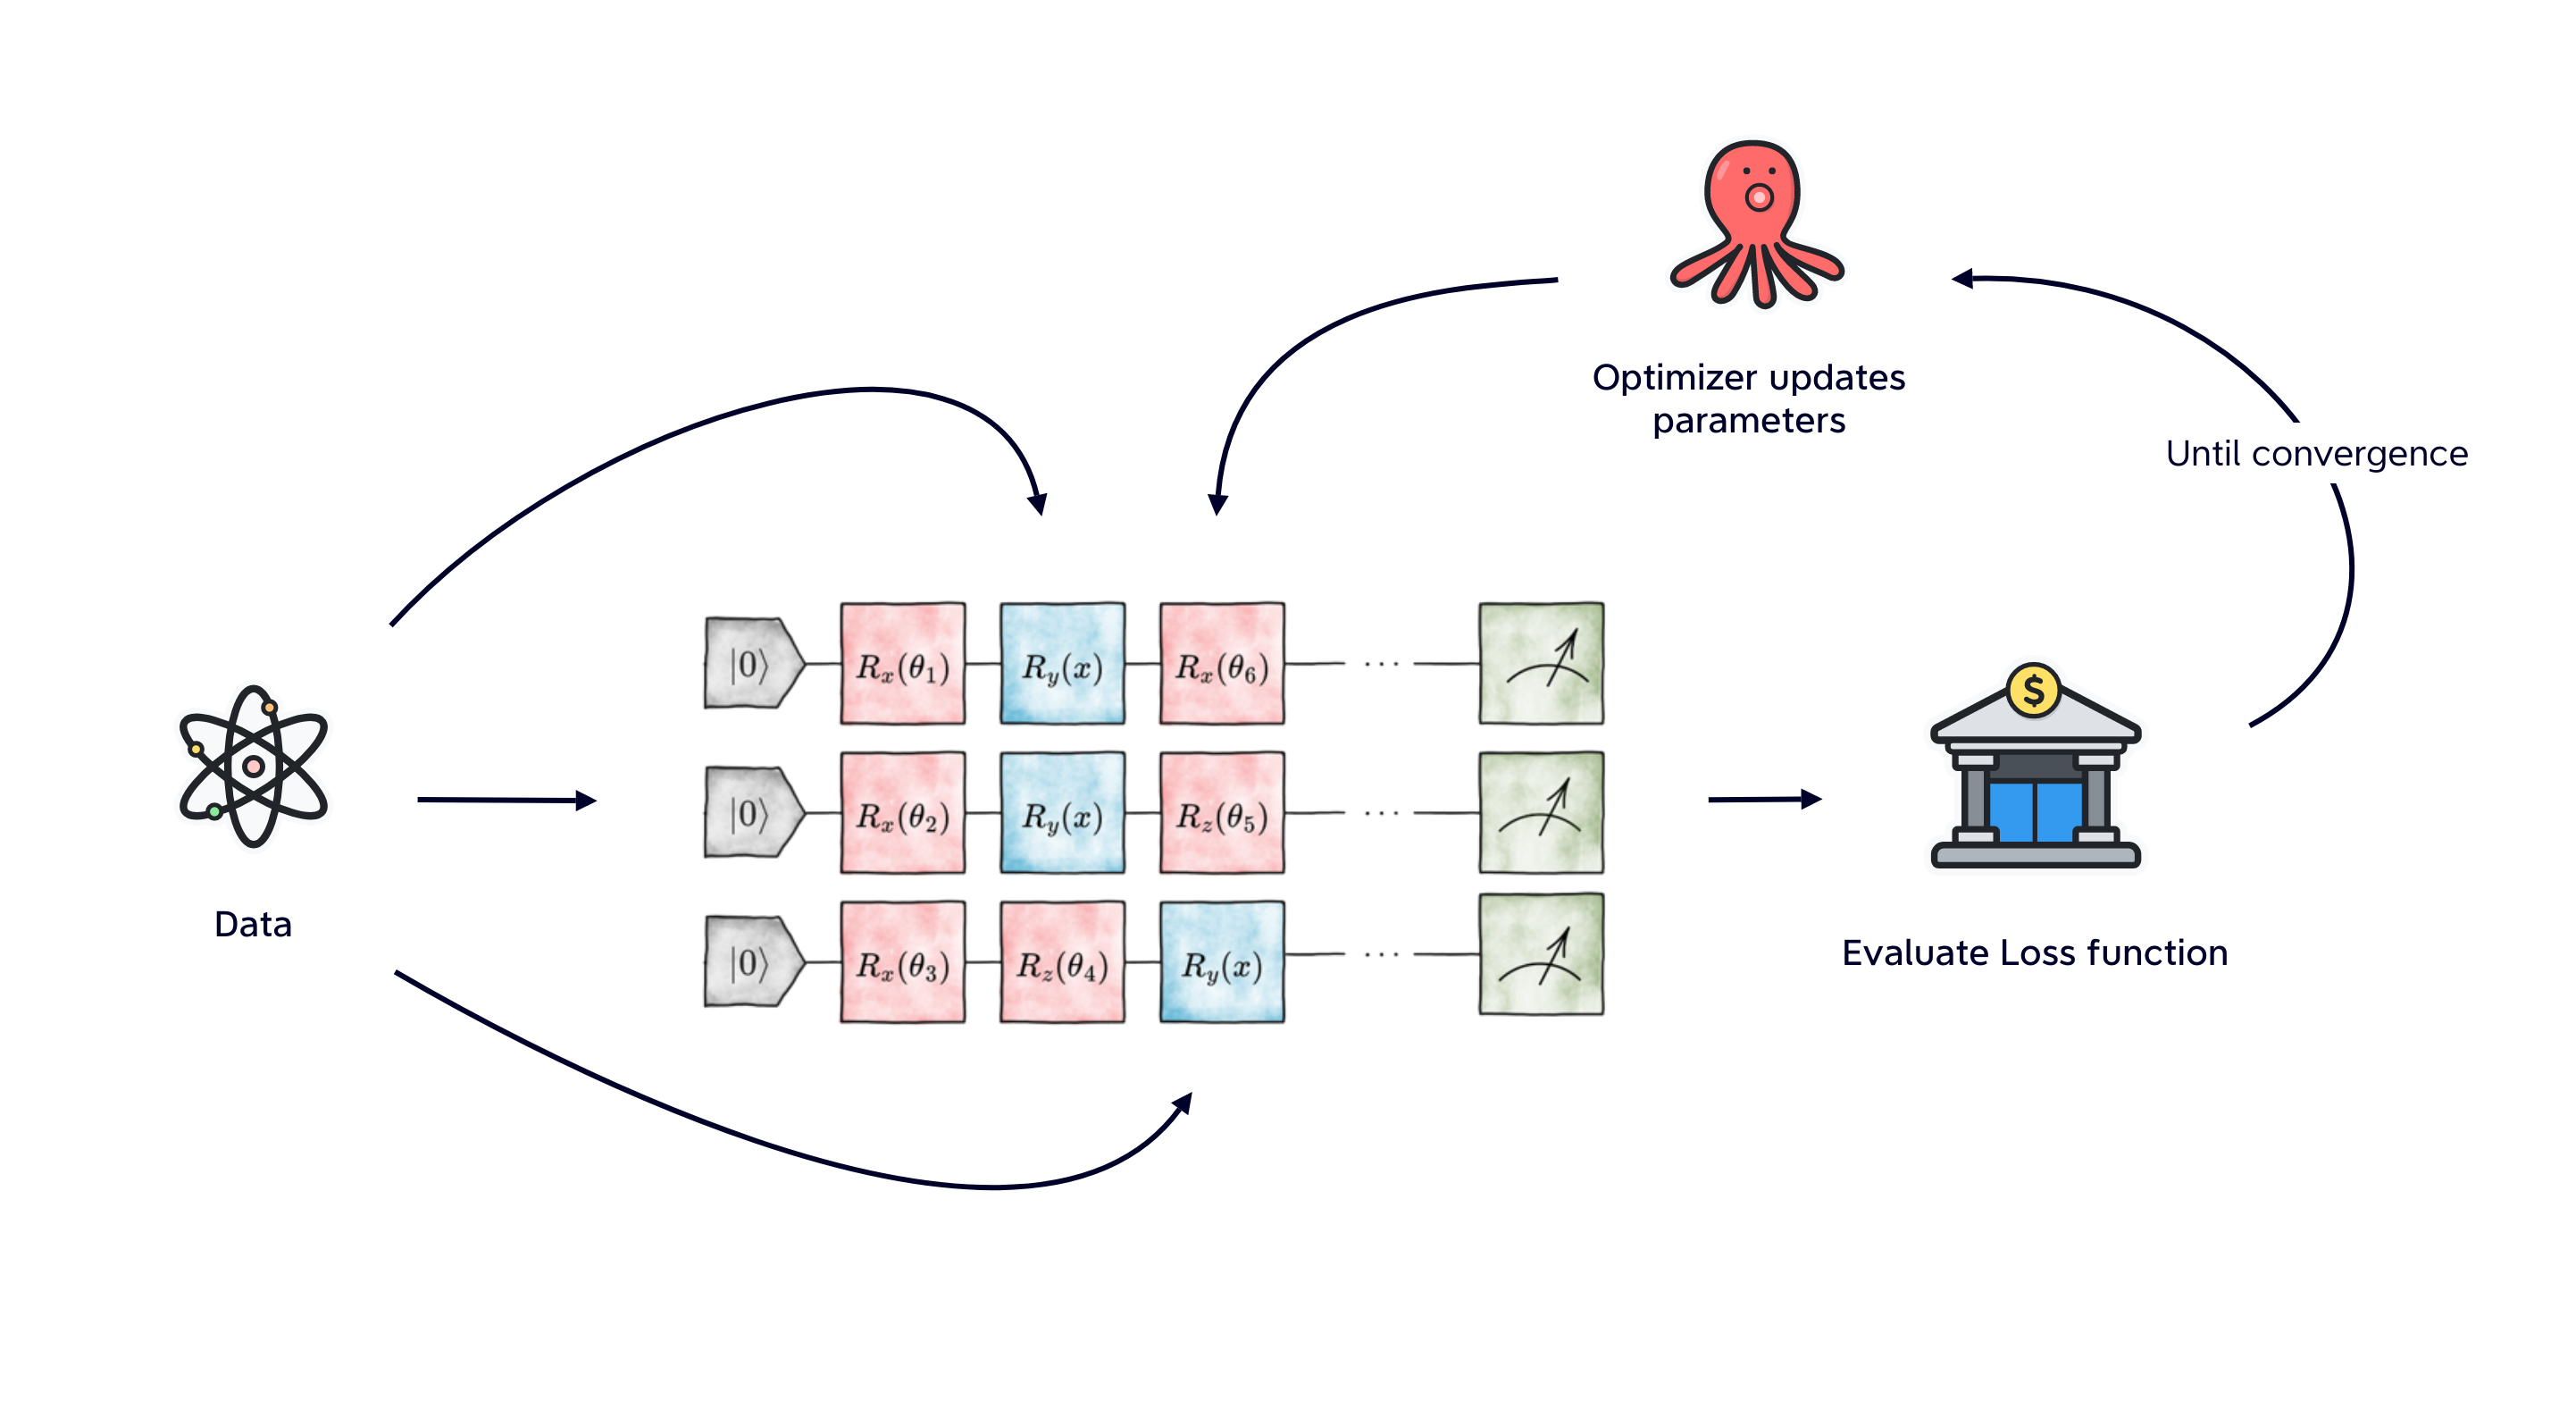
\includegraphics[width=1\textwidth]{figures/qml_scheme.png}
\end{figure}
\end{frame}

\begin{frame}{Why QML?}
\begin{multicols}{2}
\begin{itemize}
\item<2,3,4,5,6,7>[\faCartPlus] we collect \textbf{high-dimensional} data, which challenge classical models;
\item<3,4,5,6,7>[\faCodepen] an $N$-long input variable can be stored in a $\log{N}$ qubits system; 
\item<4,5,6,7>[\faLeaf ] low power consuption\only<4->{\footnote{\faBook\,\,
\href{https://doi.org/10.1038/s43588-023-00459-6}{\textit{Are quantum computers really energy efficient?}, Sophia Chen, Jun 2023}}};
\item<5,6,7>[\faCut] can \textbf{superposition} and \textbf{entanglement} be exploited to use less 
\textbf{parameters}?
\item<6,7>[\faUserSecret ] can superposition and entanglement better deal with quantum data?\only<6->{\footnote{\faBook\,\,
\href{https://arxiv.org/abs/2307.03236}{\textit{Quantum Computing for High-Energy 
Physics: State of the Art and Challenges}, A. Di Meglio et al., Jul 2023}}}\only<6->{\footnote{\faBook\,\,
\href{https://arxiv.org/abs/2307.03236}{\textit{Quantum anomaly detection in the 
latent space of proton collision events at the LHC}, K. A. Woźniak et al., Jan 2023}}}
\end{itemize}
\begin{figure}  
   \uncover<7->{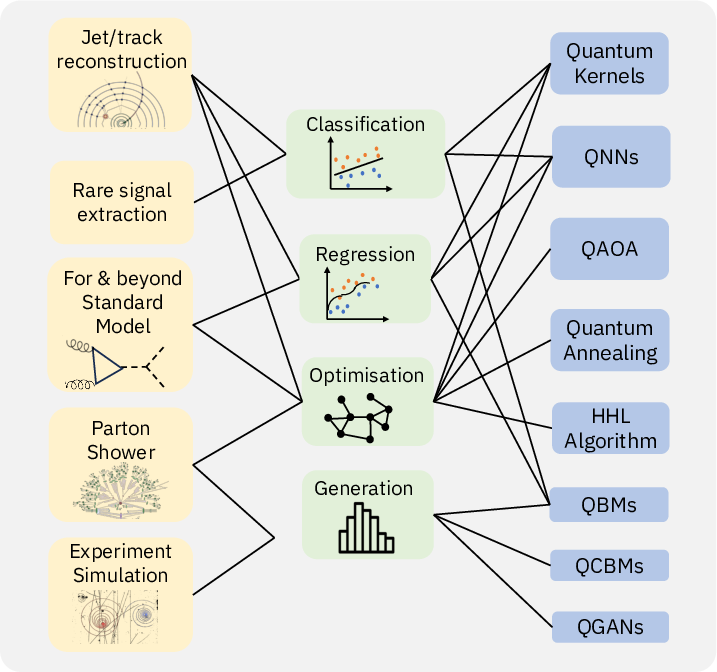
\includegraphics[width=0.5\textwidth]{figures/HEP_utils.png}}
\end{figure}
\end{multicols}
\only<2-3>{\vspace{0.8cm}}
\only<4-5>{\vspace{0.57cm}}
\end{frame}

\begin{frame}{Full-stack QML}
\begin{figure}  
    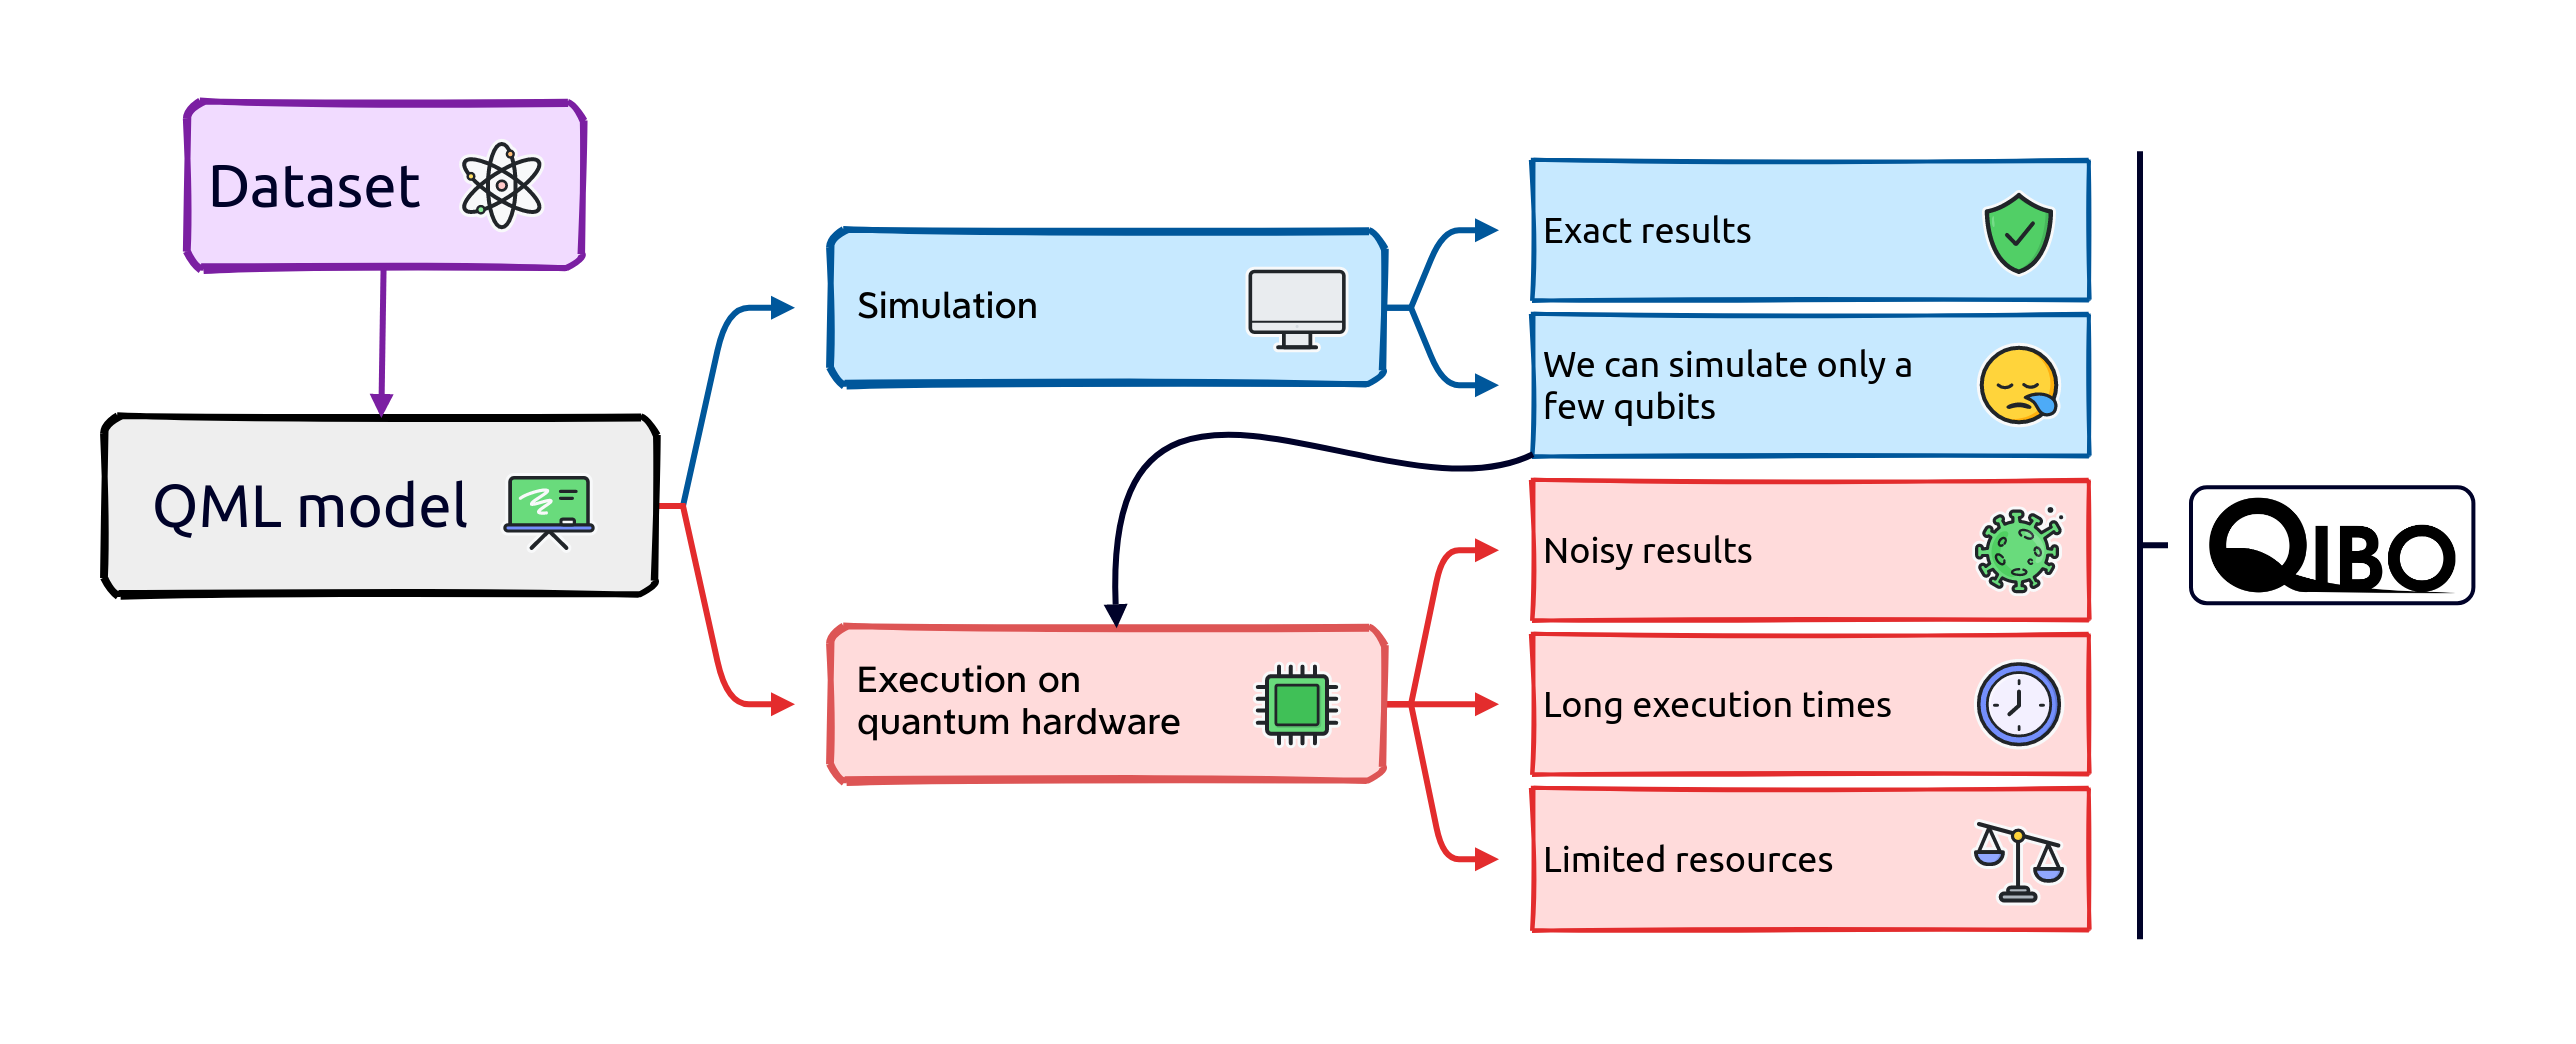
\includegraphics[width=1\textwidth]{figures/qml_onchip.png}
\end{figure}
\end{frame} 

\section{Some results}

\begin{frame}{A full-stack PDF fit \hfill \faBook\,\, \href{https://arxiv.org/abs/2308.06313}{arXiv:2308.06313}}

\begin{multicols}{2}
% column 1
\pause
\hspace{2cm}
\begin{tcolorbox}[title=High level API: Qibo, colback=blue!20]
\begin{itemize}[noitemsep]
\small
   \item[\faCode] define \textbf{prototypes} and models;
   \item[\faCode] \textbf{simulate} training and noise.
\end{itemize}
\end{tcolorbox}
\pause
\begin{tcolorbox}[title=Calibration: Qibocal, colback=yellow!20]
\begin{itemize}[noitemsep]
\small
   \item[\faCrosshairs] \textbf{calibrate} qubits;
   \item[\faCrosshairs] generate \textbf{platform configuration};
\end{itemize}
\end{tcolorbox}
\pause
\begin{tcolorbox}[title=Execution: Qibolab, colback=red!20]
\begin{itemize}[noitemsep]
\small
   \item[\faCog] allocate \textbf{calibrated} platform;
   \item[\faCog] \textbf{compile} and \textbf{transpile} circuits;
   \item[\faCog] execute and return \textbf{results}.
\end{itemize}
\end{tcolorbox}
\pause
% column 2
% PDF image
\begin{figure}  
    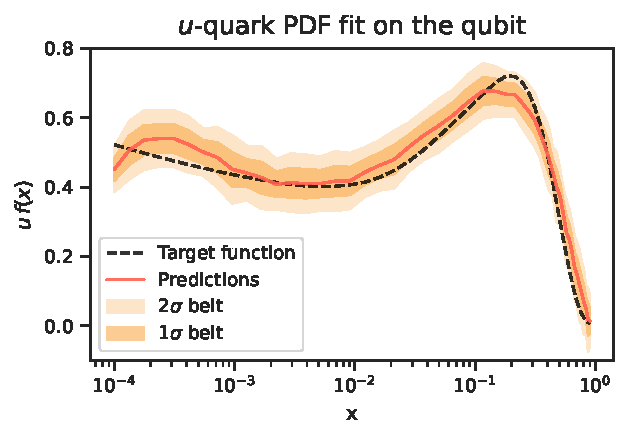
\includegraphics[width=0.5\textwidth]{figures/qpdf.pdf}
\end{figure}
% parameters
\begin{table}
\flushright
\vspace{-0.5cm}
\begin{tabular}{cc}
\hline \hline 
\textbf{Parameter} & \textbf{Value} \\
\hline 
$N_{\rm data}$ & 50 \\
$N_{\rm shots}$ & 500 \\
MSE & $\sim 10^{-3}$ \\
Electronics & Xilinx ZCU216 \\
Training time & $\sim 2$h \\
\hline \hline
\end{tabular}
\end{table}
\vspace{0.5cm}
\end{multicols}
\end{frame}

\begin{frame}{Some applications}
  \small
  %\only<2-3>{\vspace{0.1cm}}
  \begin{multicols}{2}
  \begin{itemize}
  \item<2,3,4>[-] Density estimation via Adiabatic Quantum Machine Learning,\\
  \href{https://arxiv.org/abs/2303.11346}{\faBook\,\,arXiv:2303.11346};
  \item<3,4>[-] Multi-dimensional integration using Variational Quantum Circuits,
  \href{https://arxiv.org/abs/2303.11346}{\faBook\,\,arXiv:2303.11346};
  \item<4>[-] Real-Time Quantum Error Mitigation to improve QML trainings,\\
  \href{https://arxiv.org/abs/2303.11346}{\faBook\,\,Coming soon!}
  \end{itemize}
    \begin{figure}
       \uncover<2,3,4>{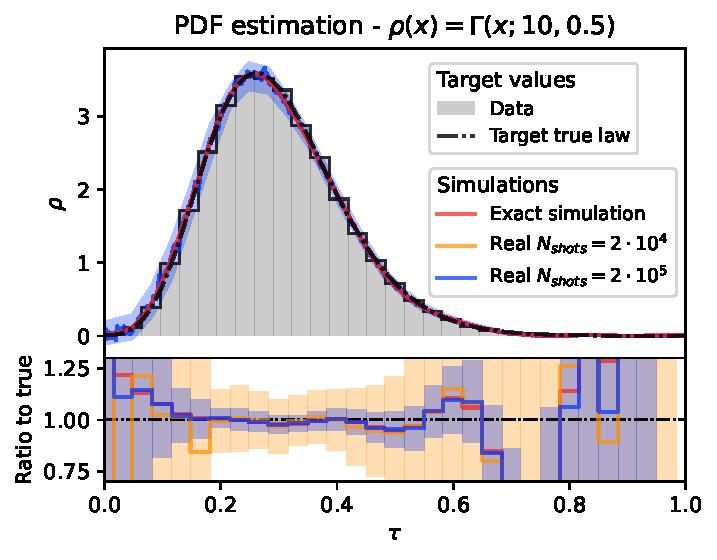
\includegraphics[width=0.45\textwidth]{figures/PDF.pdf}}%
    \end{figure}
    \begin{figure}
       \uncover<3,4>{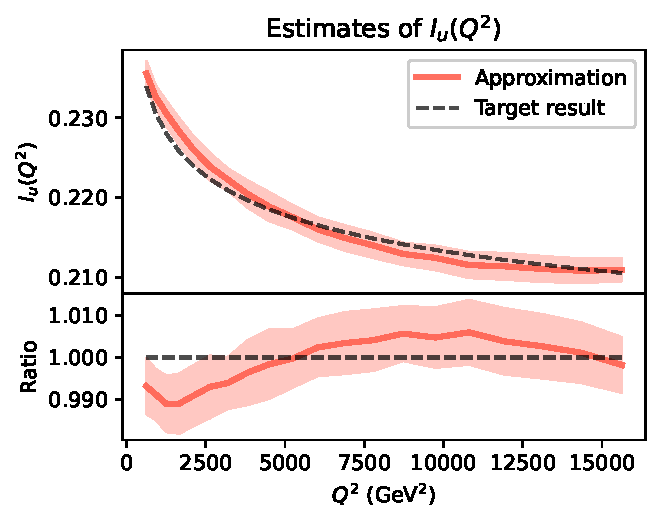
\includegraphics[width=0.45\textwidth]{figures/uquark2d.pdf}}
       \uncover<4>{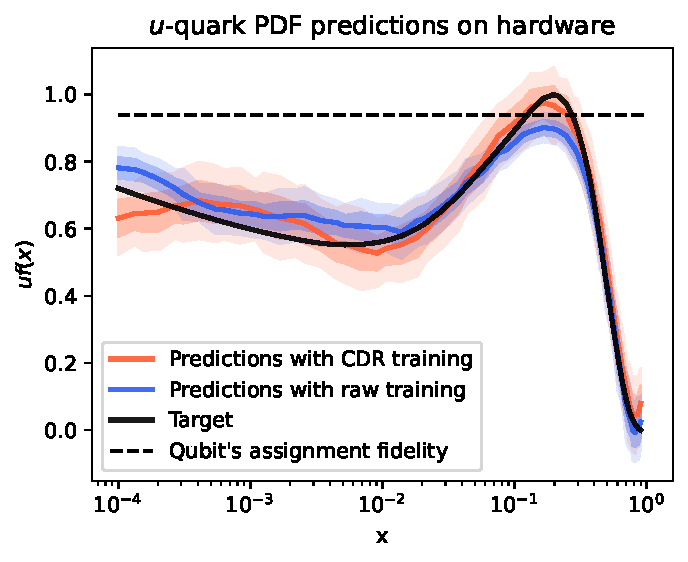
\includegraphics[width=0.45\textwidth]{figures/hardware.pdf}}%
    \end{figure}
    \end{multicols}
\end{frame}

\begin{frame}{Perspective}
\centering
\textit{``One big challenge in the next three to five years is to figure out how to 
   use the quantum hardware to improve a task in practice".} 

   Iordanis Kerenidis.
\end{frame}

\begin{frame}{}
\centering
\Large
Questions?
\end{frame}



% \begin{frame}{Simulation as first approach}
% \begin{figure}  
%     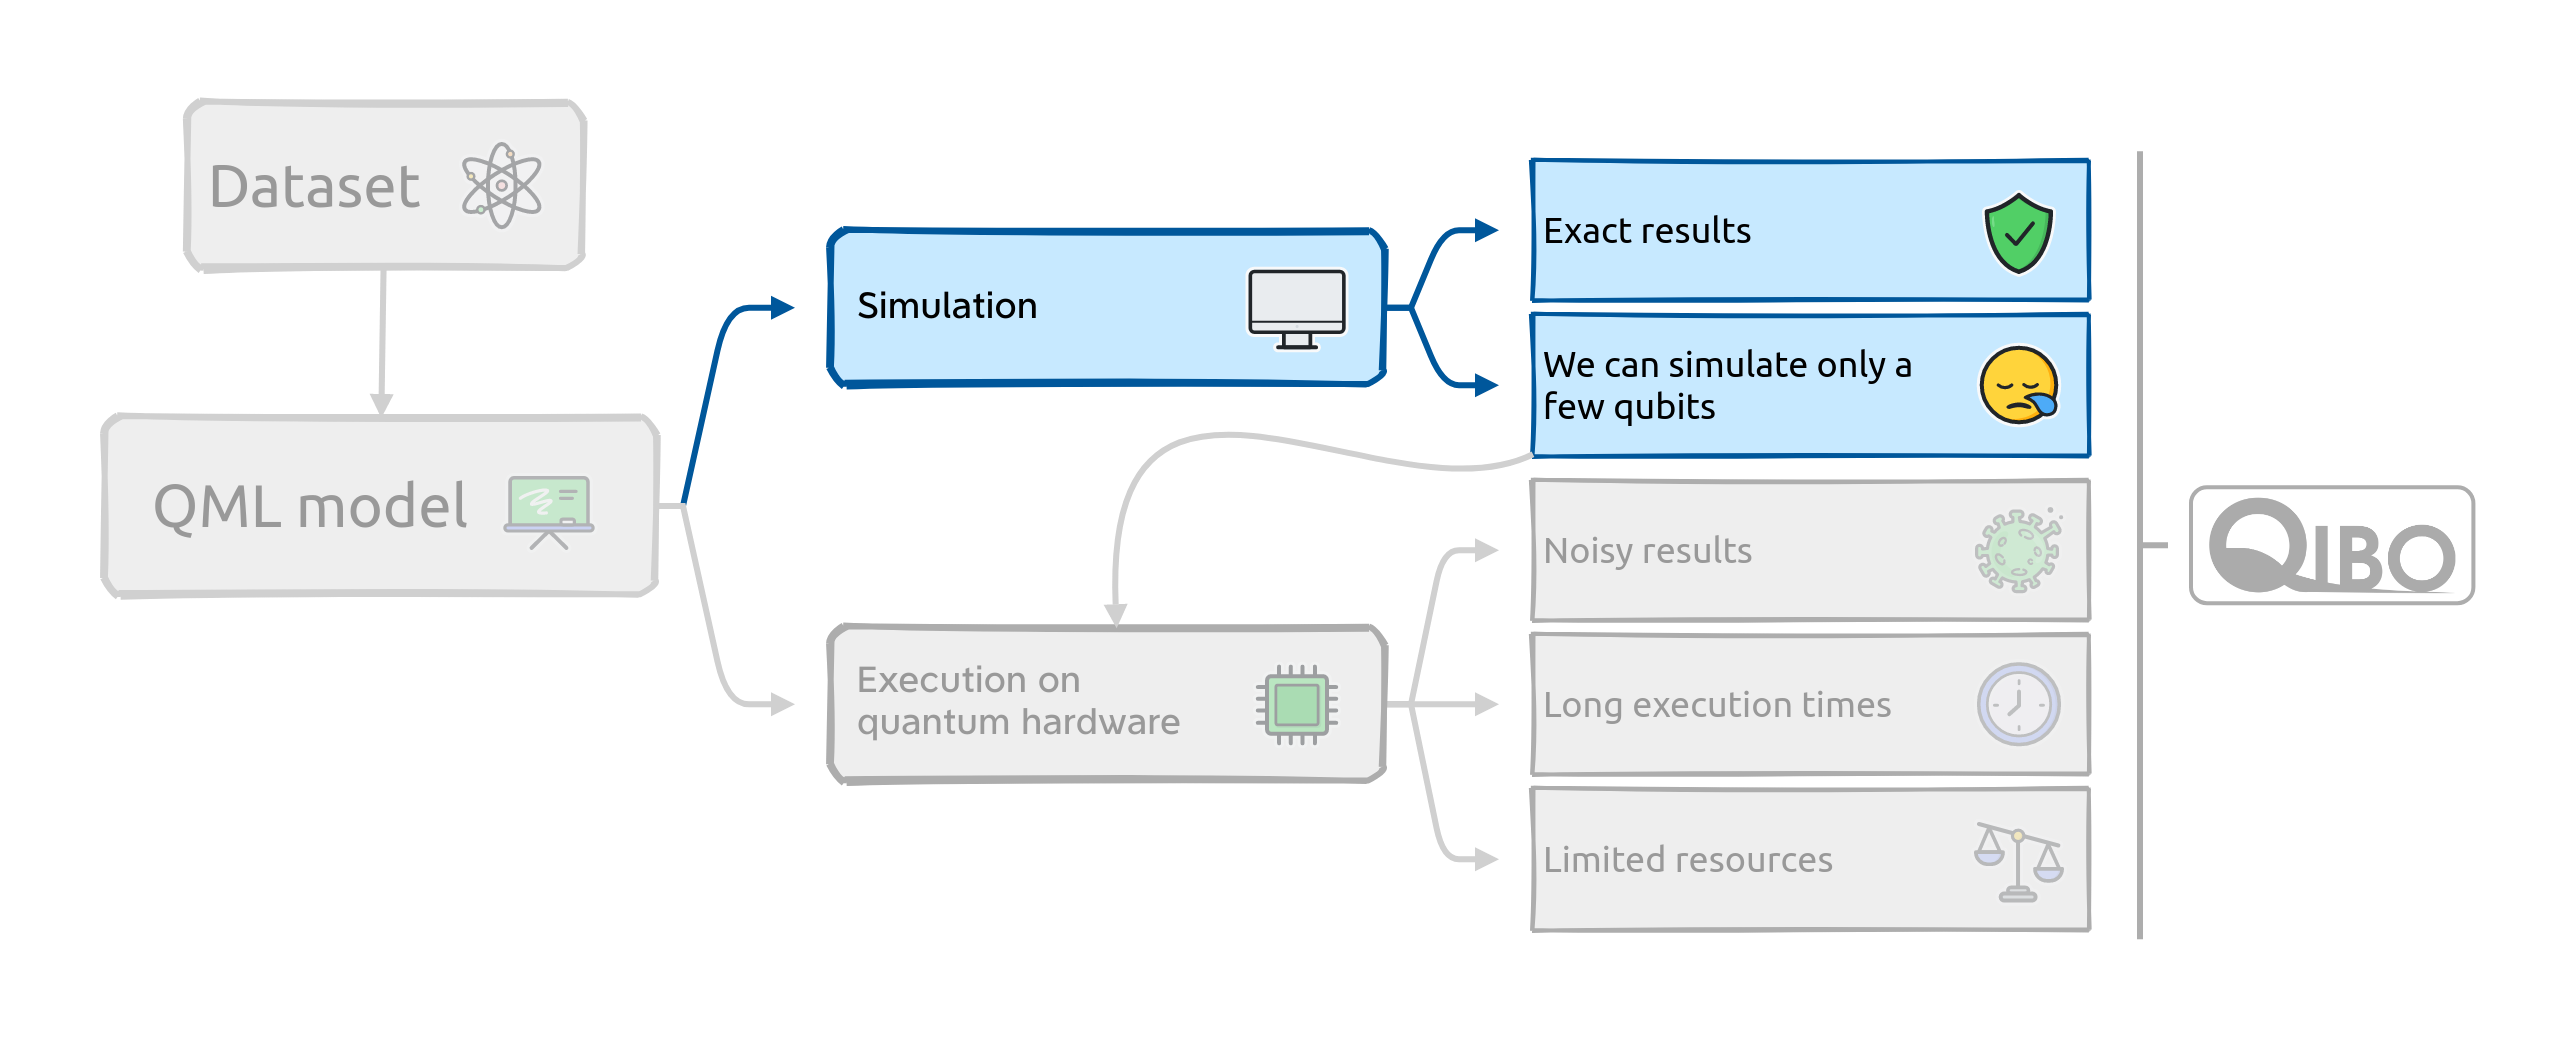
\includegraphics[width=1\textwidth]{figures/qml_sim.png}
% \end{figure}
% \end{frame}

\begin{frame}{Determining PDFs with adiabatic quantum computing}
\small
\faCrosshairs\,\, Determining Probability Density Functions (PDF).

\faFlash\,\, Algorithm's summary:
\begin{itemize}[noitemsep]
\item[1.] we optimize the parameters $\bm{\theta}$ of the following adiabatic evolution:
\begin{equation} 
H_{\rm ad}(\tau; \bm{\theta}) = [1-s(\tau; \bm{\theta})] \hat{\sigma}_x + s(\tau; \bm{\theta})\hat{\sigma}_z.
\end{equation}
we use the GS of the evolved $H_{\rm ad}$ to approximate the Cumulative
Density Function (CDF);
\item[2.] we derivate from $H_{\rm ad}$ a circuit $\mathcal{C}(\tau; \bm{\theta})$ whose action 
on the GS of $\hat{\sigma}_x$ returns $\ket{\psi(\tau)}$;
\item[3.] we compute the PDF by derivating $\mathcal{C}$ w.r.t. $\tau$ 
using the Parameter Shift Rule (PSR).
\vspace{0.05cm}
\end{itemize}
\begin{figure}  
    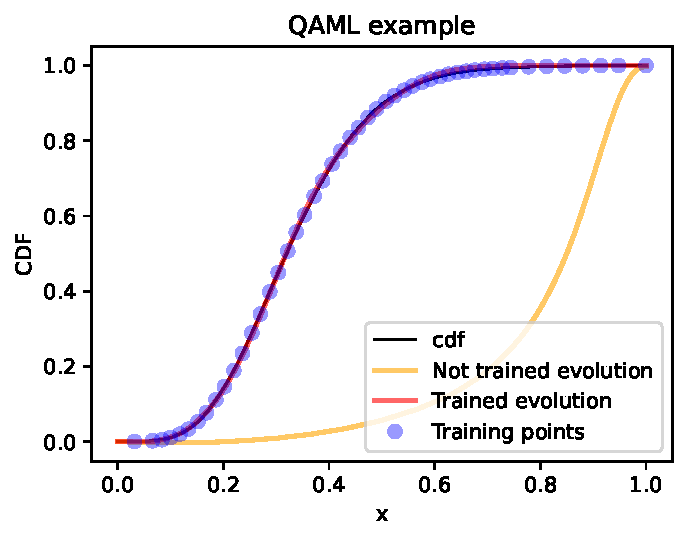
\includegraphics[width=0.5\textwidth]{figures/evolution.pdf}%
    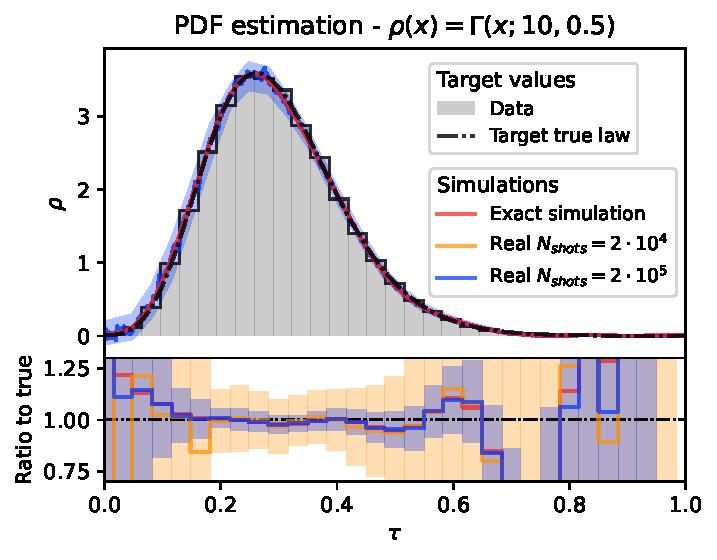
\includegraphics[width=0.5\textwidth]{figures/PDF.pdf}
\end{figure}
\end{frame}

% \begin{frame}{How does my algorithm perform on a real quantum computer?}
% \begin{figure}  
%     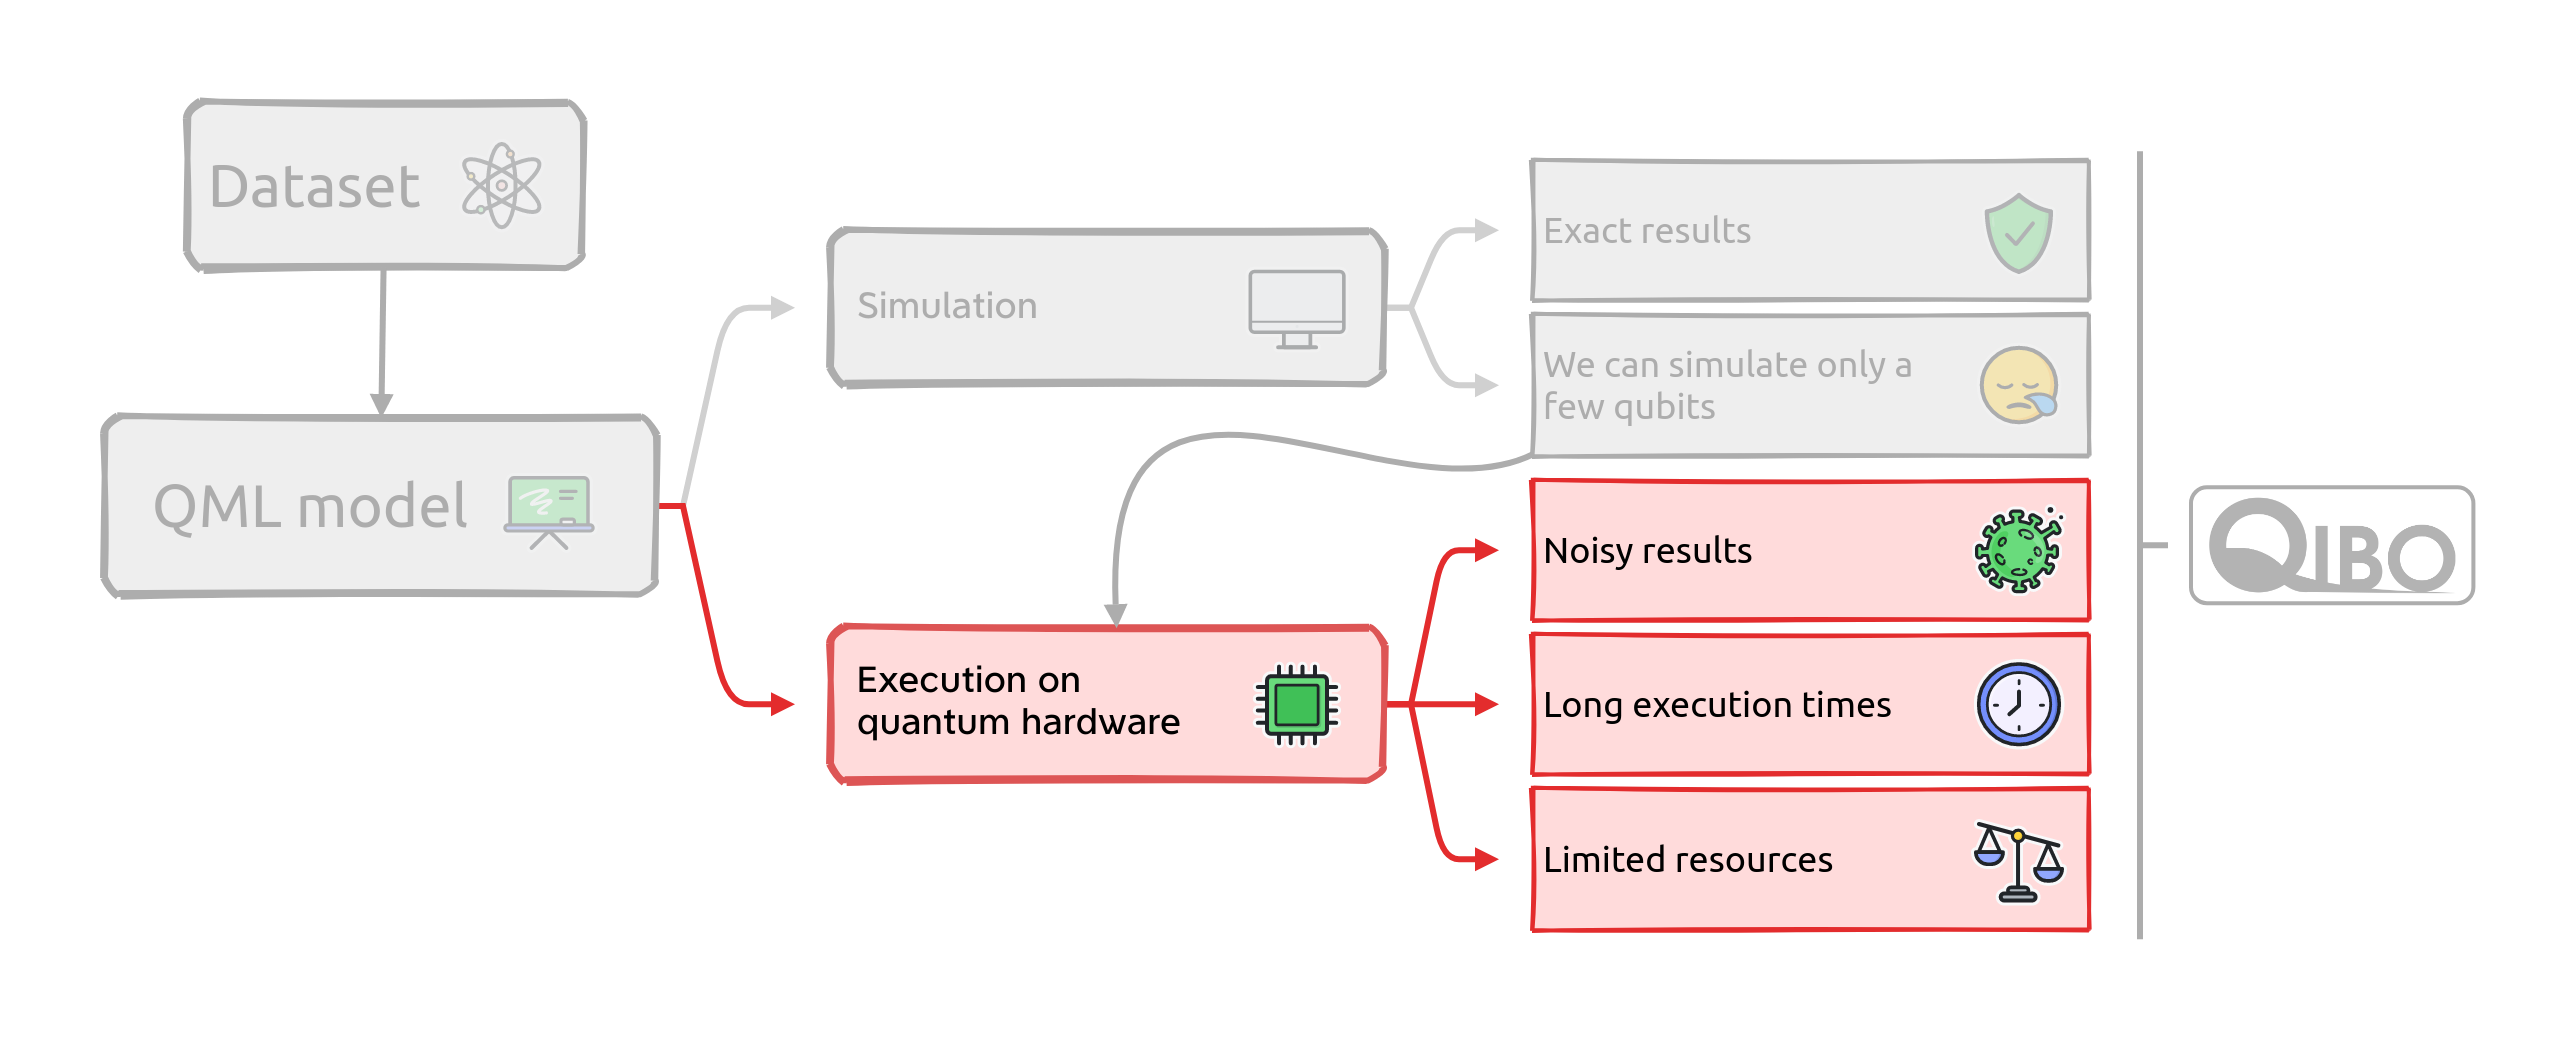
\includegraphics[width=1\textwidth]{figures/qml_hdw.png}
% \end{figure}
% \end{frame}

\begin{frame}{Multi-dimensional integration on hardware}
\small
\faCrosshairs\,\, Use Variational Quantum Circuits to calculate multi-dimensional 
integrals of the form
\begin{equation}
I(\alpha) = \int_{\bm{x}_a}^{\bm{x}_b} g(\alpha; \bm{x}) \text{d}^n \bm{x}.
\label{eq:integral}
\end{equation}

\faFlash\,\, Algorithm's summary:
\begin{itemize}[noitemsep]
\item[1.] we train the derivative of a VQC w.r.t. the integral variables $\bm{x}$ to approximate $g(\bm{x})$;
\item[2.] we compute the derivatives using the PSR, which allows the same circuit 
$\mathcal{C}$ to be used for approximating any integrand 
marginalisation and the primitive!
when varying $\alpha$.
\end{itemize}
\begin{figure}  
    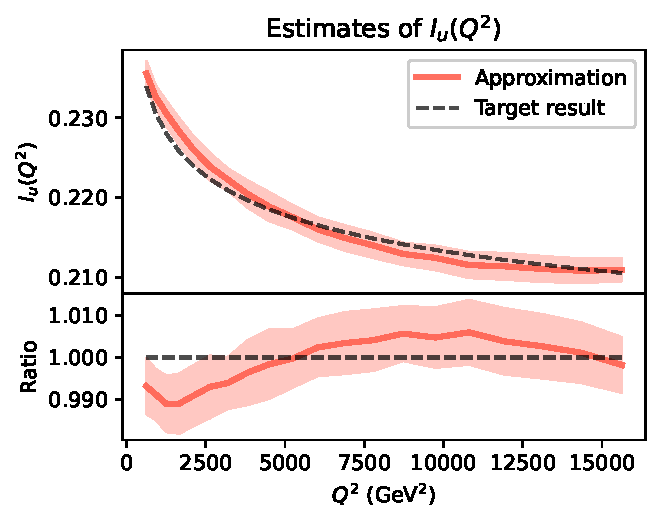
\includegraphics[width=0.5\textwidth]{figures/uquark2d.pdf}%
    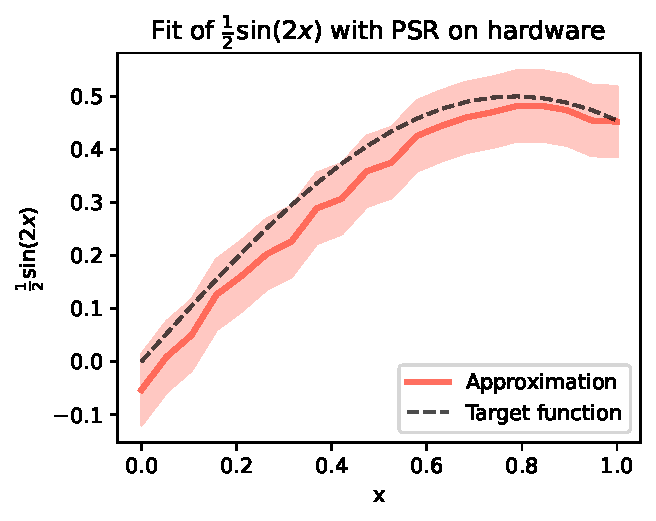
\includegraphics[width=0.5\textwidth]{figures/hardware_int.pdf}
\end{figure}
\end{frame}

% \begin{frame}{How to deal with noise?}
% \begin{figure}  
%     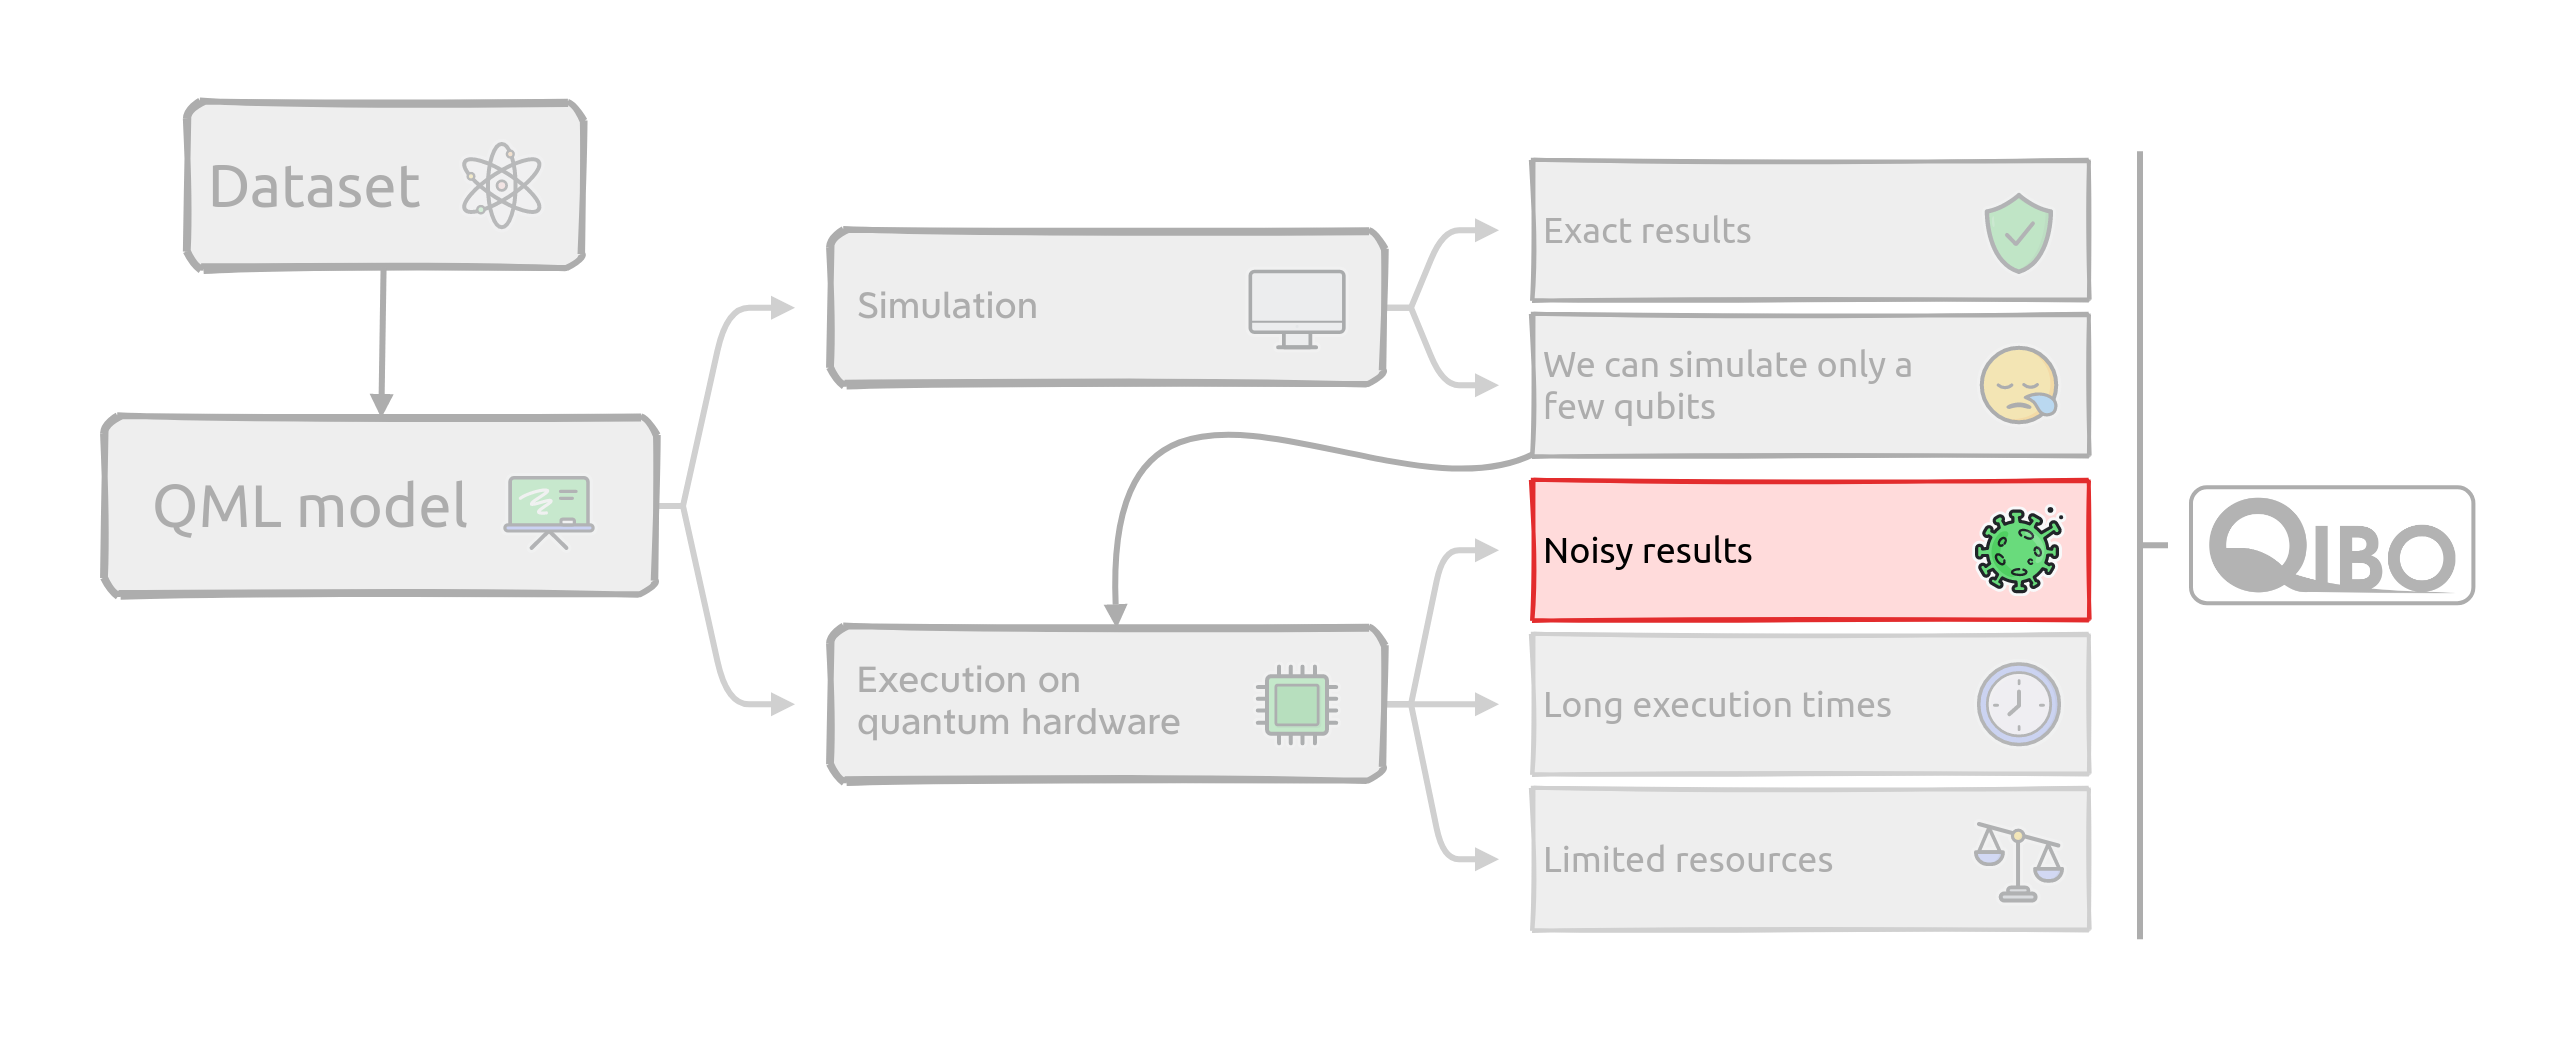
\includegraphics[width=1\textwidth]{figures/qml_qem.png}
% \end{figure}
% \end{frame}

\begin{frame}{Real time error mitigation in QML trainings}
\small
\faCrosshairs\,\,Use Error Mitigation techniques to clean up the parameters space 
during the QML training.

\faFlash\,\, Algorithm's summary:
\begin{itemize}[noitemsep]
\item[1.] we mitigate all the expected values $E$ through Clifford Data Regression (CDR):
\begin{equation}
E_{\rm mit} = \alpha_{\rm cdr} E_{\rm noisy} + \beta_{\rm cdr};
\end{equation}
\item[2.] we update $(\alpha, \beta)_{\rm cdr}$
periodically during the training in order to track the noise;
\item[3.] the mitigation removes the bounds and accelerates the training process.
\end{itemize}
\vspace{0.15cm}
\begin{figure}  
    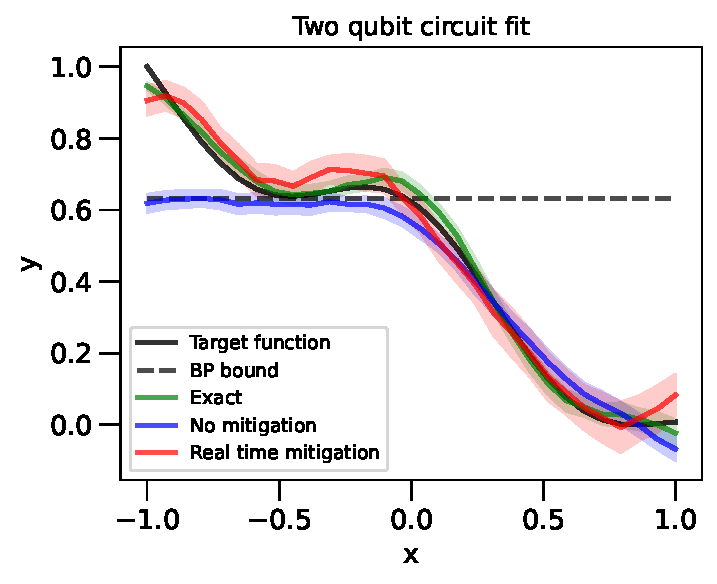
\includegraphics[width=0.5\textwidth]{figures/2qfit.pdf}%
    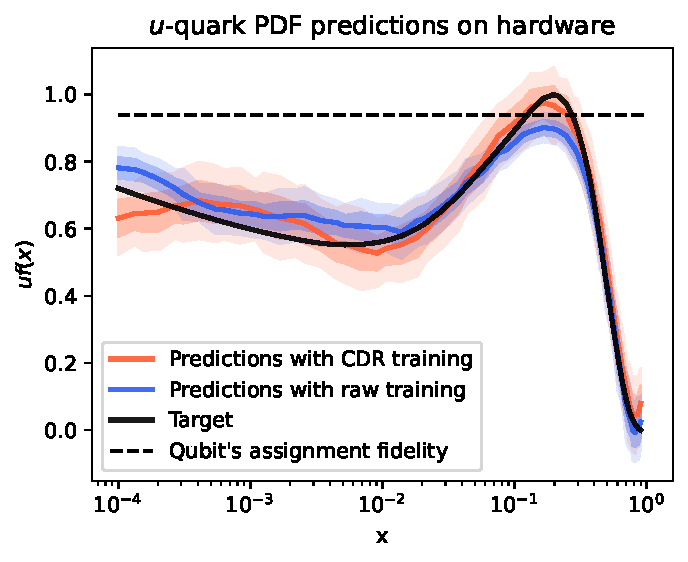
\includegraphics[width=0.5\textwidth]{figures/hardware.pdf}
\end{figure}
\end{frame}

\begin{frame}{Parameter Shift Rule}
\begin{multicols}{2}
\begin{figure}
    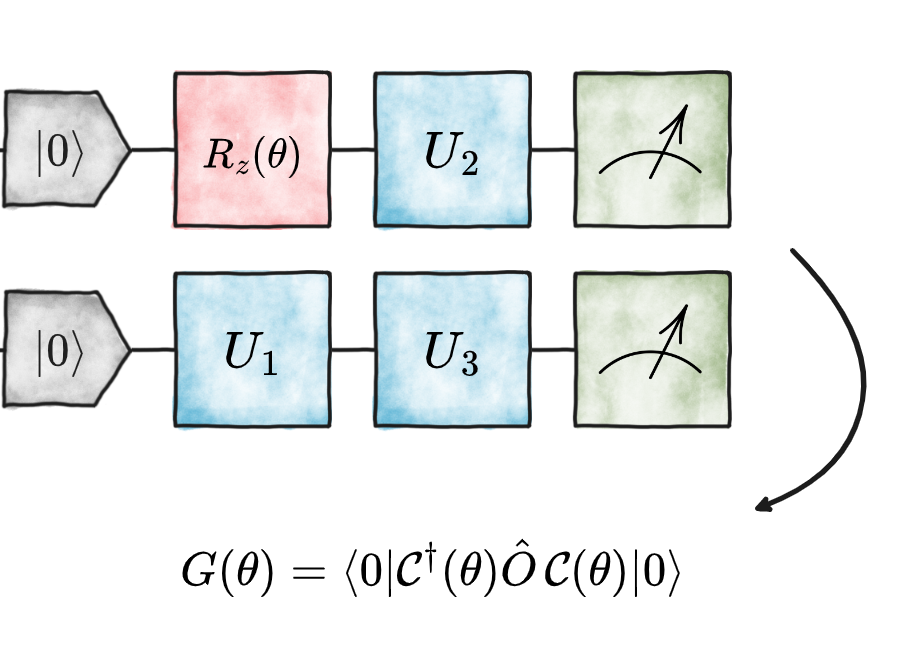
\includegraphics[width=0.45\textwidth]{figures/start.png}
\end{figure}
\begin{figure}  
    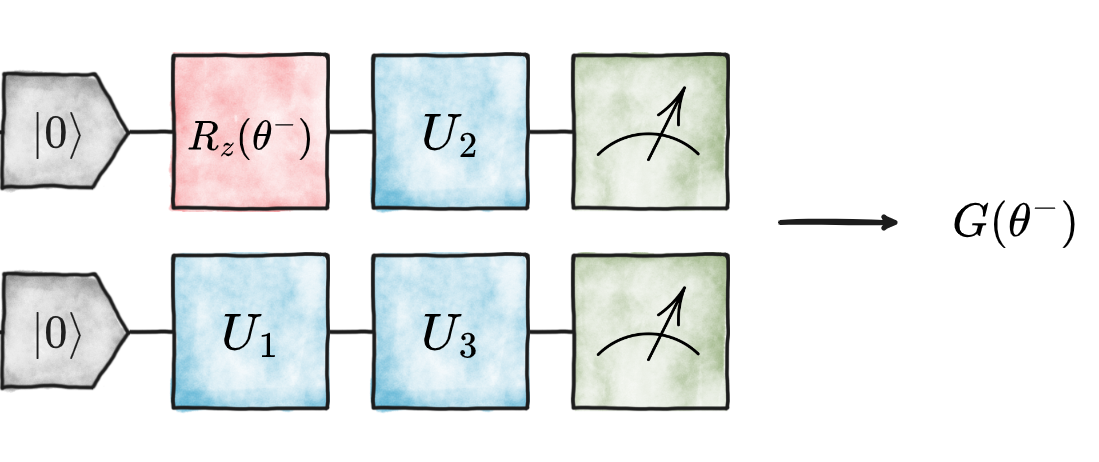
\includegraphics[width=0.5\textwidth]{figures/backward.png}
    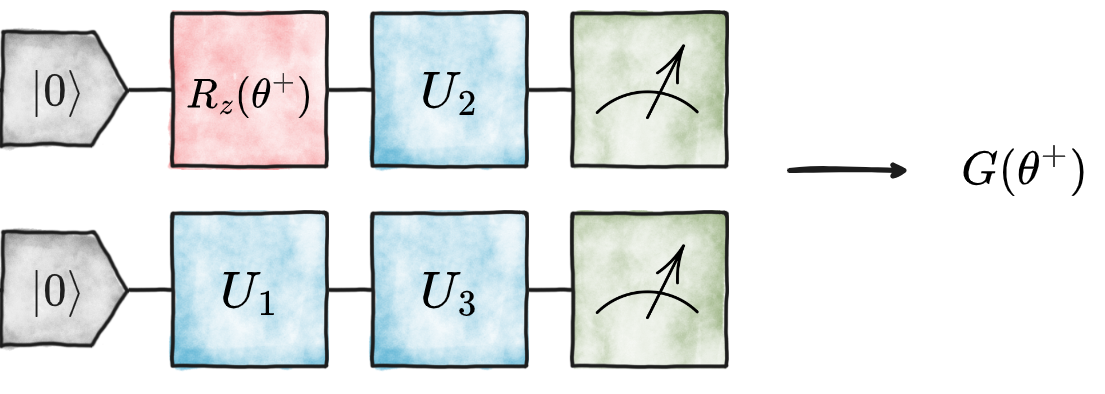
\includegraphics[width=0.5\textwidth]{figures/forward.png}
\end{figure}
\end{multicols}

The same circuit is executed twice with a shifted target parameter $\theta$, then an 
exact evaluation of the derivative is given by:
$$ \partial_\theta G = r \bigl[ G(\theta^+) - G(\theta^-) \bigr]. $$
\end{frame}

\begin{frame}{Clifford Data Regression}
\begin{figure}
    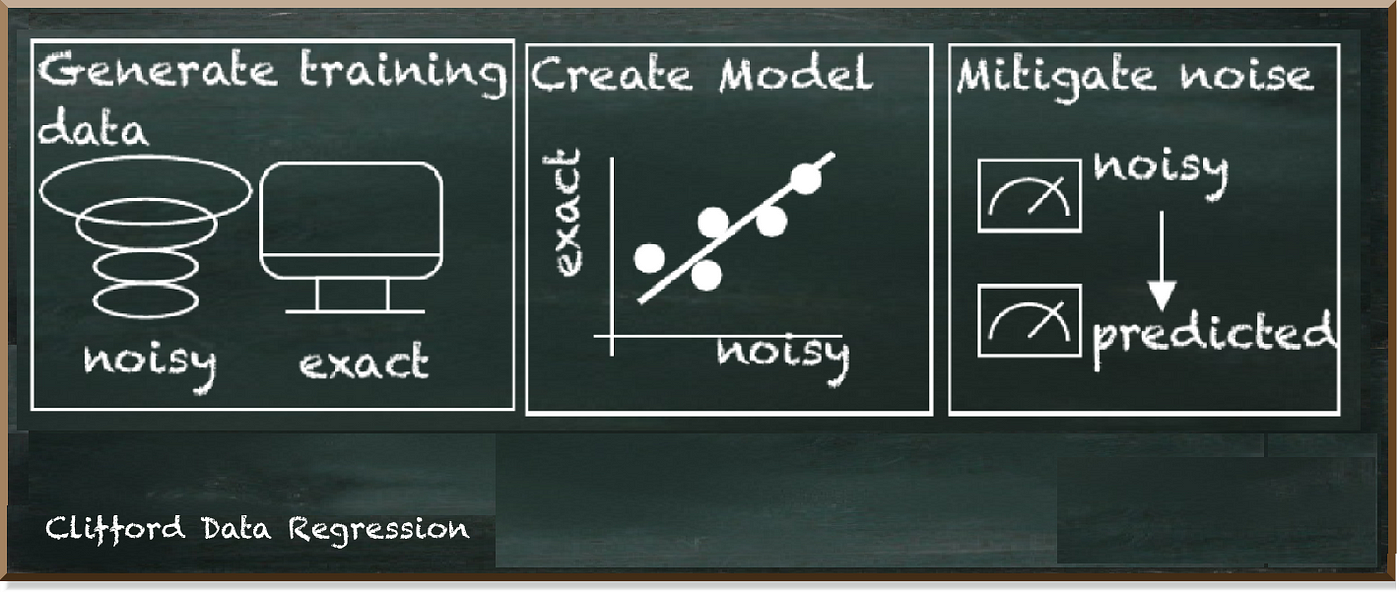
\includegraphics[width=1\textwidth]{figures/cdr.png}
    \caption{Credits: Frank Zickert.}
\end{figure}
\end{frame}

\end{document}
